\chapter{Radiative corrections}
\setcounter{chapter}{6}
\section{Optical theorem}
We have seen in Advanced Quantum Theory that tree diagrams are in general \underline{real}. So there is no imaginary parts. Need to restore perturbatively in higher-order corrections. Then the optical theorem is valid again.

S-matrix is unitary: $S^\dagger S = \id$ with $S = \id + i T$. Thus
\begin{align*}
	-i (T - T^\dagger) = T^\dagger T
\end{align*}

We take matrix element for $k_1 k_2 \rightarrow p_1 p_2$ scattering. On RHS, insert a complete set of states,
\begin{align*}
	\braket{p_1 p_2 | T^\dagger T | k_1 k_2} = \sum_n \prod_{i=1}^n \int \frac{\dd^3 q_i}{(2\pi)^3 2 E_i} \braket{p_1 p_2 | T^\dagger | q_1 \dots q_n} \braket{q_1 \dots q_n | T | k_1 k_2}
\end{align*}

Reduce $T_{fi} = (2\pi)^4 \delta^{(4)}(p_f - p_i) M_{fi}$ and omitting overall $(2\pi)^4 \delta^{(4)}(p_f - p_i)$
\begin{align*}
	-i \left[ \M(k_1 k_2 \rightarrow p_1 p_2) - \M^* (p_1 p_2 \rightarrow k_1 k_2) \right]& \\
	= \underbrace{\sum \prod_{i=1}^n \int \frac{\dd^3 q_i}{(2\pi)^3 2 E_i}}_\text{invariant phase-space volume element} & \M^*(p_1 p_2 \rightarrow q_1 \dots q_n) \M(k_1 k_2 \rightarrow q_1 \dots q_n) (2\pi)^4 \delta^{(4)}(k_1 + k_2 - \sum_i q_i)
\end{align*}

So optical theorem, for forward scattering ($p_1 = k_1, p_2 =  k_2$) reads (see \ref{math:F})
\begin{align*}
	\Im \M(k_1 k_2 \rightarrow k_1 k_2) &= 2F \sigma_\text{tot} (k_1 k_2 \rightarrow \text{anything}) \\
	2\sqrt{s} \, |f_i^\text{CMS}| &= \lambda^{\frac{1}{2}} (s, m_1^2, m_2^2)
\end{align*}

\paragraph{Optical theorem for Feynman diagrams}
Consider a specific diagram contributing to the imaginary part, e.g.~in $\phi^4$-theory.
\begin{align}
	\feynmandiagram[small, baseline=(x.base), horizontal=x to y]{
		k1[particle=\(k_1\)] -- x --[quarter left] y -- p1[particle=\(p_1\)];
		k2[particle=\(k_2\)] -- x --[quarter right] y -- p2[particle=\(p_2\)];
	};
	p_s = k_1 + k_2 = p_1 + p_2, p_s^2 = s \notag\\
	i\M(s) = \frac{\lambda^2}{2} \int \frac{\dd^4 q}{(2\pi)^4} \frac{1}{ \left[ (p_s /2 - q)^2 - M^2 +i \epsilon \right] \left[ (p_s /2 + q)^2 - M^2 + i\epsilon \right] }\label{math:M}
\end{align}

From optical theorem, $\Im \M(s < 4M^2) = 0$, so $\M(s < 4M^2) \in \R$, (since the scattering is not physical, the cross section must vanish) when regarding $\M(s)$ as an analytic function of $s$ beyond what physical S-matrix element allow.

\paragraph{Schwarz reflection principle}
If (in some region) analytic function $\M(s)$ is \underline{real} at least for a finite, non-vanishing interval $\in \R$, then
\begin{align}
	\M(s^*) = \M^* (s)
\end{align}

Hence 
$$\M(s+i\epsilon)-\M(s-i\epsilon) \equiv \text{disc} \M(s) = \M(s + i\epsilon) - \M^*(s+i\epsilon) = 2i \Im \M(s+i\epsilon)$$
\begin{center}
\tikzset{zigzag/.style={decorate, decoration=zigzag}}
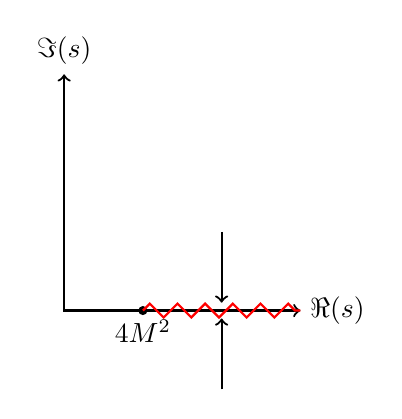
\begin{tikzpicture}[scale=1, transform shape]
	\draw [thick, <->] (0,3) -- (0,0) -- (3,0);
	\node [above] at (0,3) {$\Im(s)$};
	\node [right] at (3,0) {$\Re(s)$};
	\draw [fill] (1,0) circle [radius=0.05];
	\node [below] at (1,0) {$4M^2$};
	\draw [thick, zigzag, red] (1,0) -- (3,0);
	\draw [thick, ->] (2,1) -- (2,0.1);
	\draw [thick, ->] (2,-1) -- (2,-0.1);
\end{tikzpicture}
\end{center}

Onset of imaginary part for $s \leq 4M^2$ necessarily leads to a "branch cut", a non-trivial discontinuity in the complex energy plane. The branch cut is equivalent to $\sqrt{4M^2 - s}$. Function has discontinuity, a cut, on real axis.

How can we calculate the discontinuity ($=$ imaginary part) of the above diagram? Use centre-of-mass system $p_s = (\sqrt{s}, \pmb{0})$. Poles from propagators 
\begin{align*}
   \frac{s}{4} \mp \sqrt{s}q^0 + q^2 - M^2 + i\epsilon &= 0  \\
   \Leftrightarrow (q^0)^2 \pm \sqrt{s} q^0 + \frac{s}{4} - |\pmb{q}|^2 -M^2 + i\epsilon &= 0
\end{align*}

\begin{align*}
	& \text{First propagator} && q^0 = + \frac{\sqrt{s}}{2} \pm (\sqrt{M^2 + |\pmb{q}|^2} - i\epsilon) = +\frac{\sqrt{s}}{2} \pm (E_q - i\epsilon) \\
	& \text{Second propagator} && q^0 = -\frac{\sqrt{s}}{2} \pm (E_q - i\epsilon)
\end{align*}

\begin{center}
\tikzset{zigzag/.style={decorate, decoration=zigzag}}
\begin{tikzpicture}[scale=1, transform shape]
	\draw [thick, <->] (0,2) -- (0,0) -- (5,0);
	\draw [thick] (0,-2) -- (0,0) -- (-5,0);
	\node [above] at (0,2) {$\Im(q^0)$};
	\node [right] at (5,0) {$\Re(q^0)$};
	\node [above] at (-2,0.5) {$+\frac{\sqrt{s}}{2} - E_q + i\epsilon$};
	\draw [fill] (-2,0.5) circle [radius=0.05];
	\node [above] at (-5,0.5) {$-\frac{\sqrt{s}}{2} - E_q + i\epsilon$};
	\draw [fill] (-5,0.5) circle [radius=0.05];
	\node [below] at (2,-0.5) {$-\frac{\sqrt{s}}{2} + E_q + i\epsilon$};
	\draw [fill] (2,-0.5) circle [radius=0.05];
	\node [below] at (5,-0.5) {$+\frac{\sqrt{s}}{2} + E_q + i\epsilon$};
	\draw [fill] (5,-0.5) circle [radius=0.05];
\end{tikzpicture}
\end{center}

If we close the contour of the $q_0$ integration in the \underline{lower} half plane, we only pick up the 2 residues at $\mp \frac{\sqrt{s}}{2}+E_q -i\epsilon$. As $E_q$ is positive, only $-\frac{\sqrt{s}}{2} + E_q -i \epsilon$ from second propagator contributes to discontinuity. So pinching up the residue equivalent to replacement under $q^0$ integration
\begin{align*}
	\frac{1}{(p_s /2 + q)^2 - M^2 +i\epsilon} \longmapsto  \underbrace{-2\pi i}_{\text{orientation of contour}} \delta((p_s / 2 + q)^2 - M^2)
\end{align*}

Determine the residue of the rest at the pole at $-\frac{\sqrt{s}}{2} + E_q  - i\epsilon$
\begin{align}
	M(s) \longmapsto &-\frac{\lambda^2}{2} \int \frac{\dd^3 q}{(2\pi)^3} \frac{1}{2E_q \sqrt{s}(\sqrt{s}-2E_q)} \notag \\
	\shortintertext{With no angular dependence and using substitution (note the limits of integral also change)$\dd^3 q \rightarrow 4 \pi |\pmb{q}|^2 \dd |\pmb{q}| = 4 \pi |\pmb{q}|E_q \dd E_q$}
	& = -\frac{\lambda^2}{8\pi^2} \int^\infty_M \frac{\dd E_q \sqrt{E_q^2 - M^2}}{\sqrt{s}(\sqrt{s} - 2E_q)}  \label{math:res}
\end{align}

It has pole at $E_q = \frac{\sqrt{s}}{2}$. The second pole in \ref{math:M} at $\frac{\sqrt{s}}{2} + E_q - i\epsilon$ would produce a pole in \ref{math:res} for $E_q = -\frac{\sqrt{s}}{2}$, outside the integration range $M \leq E_q < \infty$.

\begin{itemize}
	\item for $\sqrt{s} < 2M$, \ref{math:res} is manifestly real.
	\item for $\sqrt{s} > 2M$, the pole at $E_q = \frac{\sqrt{s}}{2}$ in \ref{math:res} contributes \underline{differently} depending on $\sqrt{s}\pm i\epsilon$; difference yields discontinuity.
\end{itemize}
Use
\begin{align*}
	\frac{1}{\sqrt{s}-2E_q\pm i\epsilon} = \underbrace{\frac{P}{\sqrt{s} - 2 E_q}}_{\text{real}} \underbrace{\mp i\pi \delta(\sqrt{s} - 2 E_q)}_{\text{yields discontinuity}}
\end{align*}

So for calculation of the discontinuity, have replacement 
\begin{align*}
	\frac{1}{(p_s/2 - q)^2 - M^2 + i\epsilon} \longmapsto -2\pi i \delta((p_s/2 -q)^2 - M^2)
\end{align*}
for other propagator too!

\paragraph{Cuthosky rules (1960)} replace cut propagator according to 
\begin{align}
	\frac{1}{p^2 - M^2 + i\epsilon} \longmapsto -2\pi  i \delta(p^2 - M^2)
\end{align}
to calculate discontinuity across the cut!

Calculation completed:
\begin{align*}
	\text{disc} \left(	
		\feynmandiagram[small, baseline=(x.base), horizontal=x to y]{
			k1 -- x --[quarter left] y -- p1;
			k2 -- x --[quarter right] y -- p2;
		};
	\right )
	 &= i\frac{\lambda^2}{2} \int \frac{\dd^4 q}{(2\pi)^4} 2\pi \delta(q^2 - M^2) 2\pi \delta((p_s - q)^2 - M^2) \\
	 \shortintertext{using $\dd^4 q = \dd q^0 \dd q |q|^2 \dd \Omega_q$ and $(p_s - q)^2 - M^2 = s - 2\sqrt{s}q^0$}
	 &= \frac{\lambda^2}{2} \frac{i}{4\pi^2} \int \frac{|q|^2 \dd |q| \dd \Omega_q}{2q^0} \delta(s - 2\sqrt{s}q^0) \\
	 &= \frac{\lambda^2}{2} \frac{i}{8\pi^2} \int \sqrt{(q^0)^0 - M^2} \dd q^0 \dd \Omega_q \delta(s - 2\sqrt{s}q^0) \\
	 &= \frac{\lambda^2}{2} \frac{i}{8\pi^2} \frac{\sqrt{s/4 - M^2}}{2\sqrt{s}} \int \dd \Omega_q \\
	 &= \frac{\lambda^2}{2} \frac{i}{8\pi} \sqrt{1 - \frac{4M^2}{s}} \\
	\text{Im}\M &= \frac{\lambda^2}{4} \frac{1}{8\pi} \sqrt{1 - \frac{4M^2}{s}}
\end{align*}
Note $\sigma = \frac{\lambda^2}{32\pi}$ and $2F = s \sqrt{1-\frac{4M^2}{s}}$. Thus optical theorem is still valid.

We can do more. Construct the complete $\M(s)$ from $\Im\M(s)$ through a \underline{dispersion relation}!

\begin{center}
\tikzset{zigzag/.style={decorate, decoration=zigzag}}
\usetikzlibrary{decorations.markings}
\tikzset{decoration={
    markings,
    mark=at position 0.5 with {\arrow{>}}}}
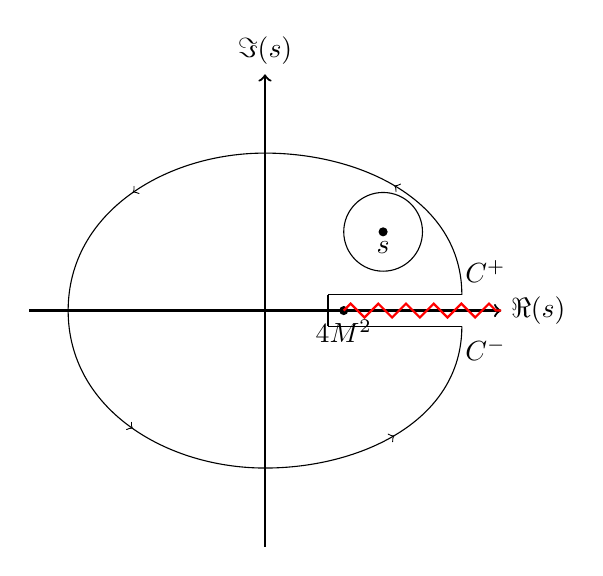
\begin{tikzpicture}[scale=1, transform shape]
	\draw [thick, <->] (0,3) -- (0,0) -- (3,0);
	\draw [thick, -] (0,-3) -- (0,0) -- (-3,0);
	\node [above] at (0,3) {$\Im(s)$};
	\node [right] at (3,0) {$\Re(s)$};
	\draw [fill] (1,0) circle [radius=0.05];
	\node [below] at (1,0) {$4M^2$};
	\draw [thick, zigzag, red] (1,0) -- (3,0);

	\draw [fill] (1.5,1) circle [radius=0.05];
	\draw (1.5,1) circle [radius=0.5];
	\node [below] at (1.5,1) {$s$};
	\draw[postaction={decorate}] (2.5,0.2) to [out=90, in=0] (0,2);
	\draw[postaction={decorate}] (0,2) to [out=-180, in=90] (-2.5,0);
	\draw[postaction={decorate}] (0,-2) to [out=0, in=-90] (2.5,-0.2);
	\draw[postaction={decorate}] (-2.5,0) to [out=-90, in=180] (0,-2) ;

	\draw (0.8,0.2) -- (2.5,0.2);
	\draw (0.8,-0.2) -- (2.5,-0.2);
	\draw (0.8, 0.2) -- (0.8, -0.2);

	\node at (2.8,0.5) {$C^+$};
	\node at (2.8,-0.5) {$C^-$};
\end{tikzpicture}
\end{center}

Use Cauchy's theorem:
\begin{align}
	\M(s) &= \frac{1}{2\pi i} \oint \frac{\M(z)\dd z}{z-s} \\
	\shortintertext{dropping the large circle}
		  &\longmapsto  \frac{1}{2\pi i }\int_{C_+ + C_-} \frac{\M(z)\dd z}{z-s}\notag\\
	&= \frac{1}{2 \pi i} \left[ \int^\infty_{4M^2}\frac{M(z+i\epsilon)\dd z}{z-s} - \int^\infty_{4M^2}\frac{M(z-i\epsilon)\dd z}{z-s} \right] \notag\\
	&= \frac{1}{2\pi i }\int^\infty_{4M^2} \frac{\text{disc}\M(z)\dd z}{z -s } \notag\\
	&= \frac{1}{\pi} \int^\infty_{4M^2} \frac{\Im\M(z) \dd z}{z-s} 
\end{align}

Repeat the exercise for $\frac{\M(s)-\M(0)}{s}$ (no pole introduced!).
\begin{align*}
	\Im \left( \frac{\M(s)-\M(0)}{s} \right) &= \frac{\Im\M(s)}{s} \\
	\M(s) - \M(0) &= \frac{s}{\pi} \int^\infty_{4M^2} \frac{\Im\M(z)\dd z}{z(z-s)} \\
				  &= \frac{\lambda^2}{2} \frac{s}{(4\pi)^2} \int^\infty_{4M^2} \frac{\dd z}{z(z-s)} \sqrt{1-\frac{4M^2}{z}} \\
	\shortintertext{using $\sigma = \sqrt{1-\frac{4M^2}{s}}$ and $\zeta = \sqrt{1 - \frac{4M^2}{z}}$}
				&= \frac{\lambda^2}{2}\frac{1}{8\pi^2} \int^1_0 \frac{\zeta^2}{\zeta^2 - \sigma^2} \dd \zeta \\
				&= \frac{\lambda^2}{2}
	\begin{cases}
		\frac{1}{8\pi^2} \left( 1 -\frac{\sigma}{2}\log{\frac{\sigma+1}{\sigma-1}} \right) & s < 0 \Leftrightarrow \sigma > 1 \\
		\frac{1}{8\pi^2} \left( 1- \sqrt{-\sigma^2} \arctan{\frac{1}{\sqrt{-\sigma^2}}} \right) & 0 < s < 4M^2, \sigma^2 < 0 \\
		\frac{1}{8\pi^2} \left( 1 - \frac{\sigma}{2}\log{\frac{1+\sigma}{1-\sigma}} + \frac{\textcolor{red}{i}\sigma}{16\pi} \right) & s > M^2, 0 < \sigma < 1
	\end{cases}
\end{align*}

\paragraph{Note} We are going to calculate this diagram again, noticing that $\int \frac{\dd^4 q}{(q^2 \dots)(q^2 \dots)}$ is logarithmically divergent! The above representation demonstrates that this divergence resides in $M(0)$!

\section{Field-strength renormalization}
What is structure of the propagator $\braket{\Omega | T\phi(x)\phi(y) | \Omega}$ at higher orders? At lower order
\begin{align*}
	\feynmandiagram[small, horizontal=a to b]{a --[fermion, edge label=\(p\)]b;};
	= \frac{i}{p^2 - M^2 + i\epsilon}
\end{align*}
Beyond this the propagator is not a simple pole. In $\phi^3$-theory 
\feynmandiagram[layered layout, small, horizontal=a to b, baseline=(a.base)]{
	a -- x;
	x --[half left] y;
	x --[half right] y;
	y -- b;
};
branch cuts are at $p^2 \leq 4M^2$.
In $\phi^4$-theory
\feynmandiagram[layered layout, small, horizontal=a to b, baseline=(a.base)]{
	a -- x;
	x --[half left] y;
	x --[half right] y;
	x -- y;
	y -- b;
};	
branch cuts are at $p^2 \leq 9M^2$. To induce cuts in the analytic structure.

Insert complete set of intermediate states ($x^0 > y^0$)
\begin{align*}
	\braket{\Omega | T\phi(x)\phi(y) | \Omega} = \sum_\lambda \int \frac{\dd^3 p}{(2\pi)^3 2E_p(\lambda)} \braket{\Omega | \phi(x) | \lambda_{\pmb{p}}} \braket{\lambda_{\pmb{p}} | \phi(y) | \Omega}
\end{align*}
with
\begin{itemize}[label={}]
	\item $\lambda$ multi-particle state
	\item $\lambda_0$ "rest frame", i.e.~$\hat{\pmb{P}}\ket{\lambda_0} = 0$
	\item $\lambda_{\pmb{p}}$ boosted to momentum $\pmb{p}$
\end{itemize}

Call energy of $\lambda_0 = m_\lambda$. From single particle to multi particle $E_{\pmb{p}}(\lambda) = \sqrt{m^2_\lambda + |\pmb{p}|^2}$.

\begin{align*}
	\braket{\Omega | \phi(x) | \lambda_{\pmb{p}}} &= \braket{\Omega| e^{i\hat{P}x} \phi(0) e^{-i\hat{P}x}|\lambda_{\pmb{p}}}	\\
									   &= \left. \braket{\Omega| \phi(0) | \lambda_{\pmb{p}}} e^{-ipx} \right\rvert_{p^0 = E_{\pmb{p}}} \\
									   \shortintertext{$\Omega$ and $\phi(0)$ are invariant under momentum boost}
									   &= \left. \braket{\Omega| \phi(0) | \lambda_{0}} e^{-ipx} \right\rvert_{p^0 = E_{\pmb{p}}} \\
\end{align*}

\begin{align}
	\braket{\Omega | T\phi(x)\phi(y) | \Omega} &= \sum_\lambda \int \frac{\dd^3 p}{(2\pi)^3 2E_p(\lambda)} e^{-ip(x-y)} |\braket{\Omega| \phi(0) | \lambda_0 }|^2 \\
											   &= \sum_\lambda \underbrace{\int \frac{\dd^4 p}{(2\pi)^4} \frac{i}{p^2 - m^2_\lambda + i\epsilon} e^{-ip(x-y)}}_{D_F(x-y;m^2_\lambda) \text{ when combined with } y^0 > x^0} |\braket{\Omega| \phi(0) | \lambda_0 }|^2 \\ 
\end{align}

Formally write this as 
\begin{align}
	\braket{\Omega | T\phi(x)\phi(y) | \Omega} = \int^\infty_0 \frac{\dd s}{2\pi} \rho(s) D_F(x-y;s)
\end{align}
with $\rho(s)$ the spectral density function.
\begin{align}
	\rho(s) \defeq \sum_\lambda (2\pi) \delta(s - m_\lambda^2) \left| \braket{\Omega | \phi(0) | \lambda_0} \right|^2
\end{align}

A typical spectral function looks like
\begin{figure}[htpb]
\begin{center}
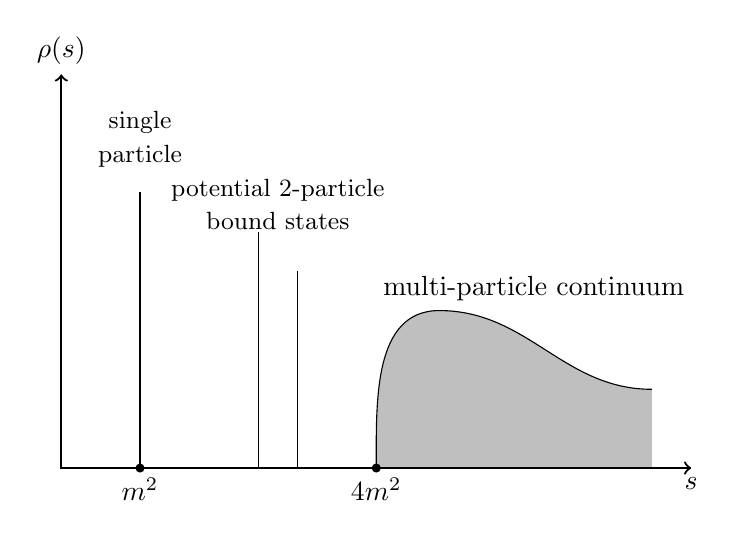
\begin{tikzpicture}[scale=1, transform shape]
	\draw [fill] (1,0) circle [radius=0.05];
	\node [below] at (1,0) {$m^2$};
	\draw (1,3.5) -- (1,0);
	\node [above, align=center] at (1,3.7) {\small single\\ \small particle};

	\draw (3,2.5) -- (3,0);
	\draw (2.5,3) -- (2.5,0);
	\node [above, align=center] at (2.75, 2.9) {\small potential 2-particle \\ \small bound states};

	\draw [draw opacity=0, fill=lightgray] (4,0) to [out=90, in=180] (4.8,2) to [out=0, in=180] (7.5,1) -- (7.5,0) ;
	\draw (4,0) to [out=90, in=180] (4.8,2) to [out=0, in=180] (7.5,1);
	\draw [fill] (4,0) circle [radius=0.05];
	\node [below] at (4,0) {$4m^2$};
	\node [above] at (6, 2) {multi-particle continuum};

	\draw [thick, <->] (0,5) -- (0,0) -- (8,0);	
	\node [above] at (0,5) {$\rho(s)$};
	\node [below] at (8,0) {$s$};
\end{tikzpicture}
\end{center}
\caption{typical spectral function}
\label{fig:specFunc}
\end{figure}

Single particle contribution
\begin{align}
	\rho(s) = 2\pi \delta(s-m^2)Z + (\text{contributions} \geq 4m^2)
\end{align}
with $Z = \left| \braket{\Omega | \phi(0) | \lambda_{0}}\right|^2$ the field-strength renormalization factor. 

Fourier transforming two-point function
\begin{align*}
	&\int \dd^4 x e^{ipx} \braket{\Omega | T\phi(x)\phi(0) | \Omega} \\
	=& \int^\infty_0 \frac{\dd s}{2\pi} \rho(s) \frac{i}{p^2 - s + i\epsilon} \\
	=& \frac{iZ}{p^2 - m^2 + i\epsilon} + \int^\infty_{\sim 4m^2} \frac{\dd s}{2\pi} \rho(s) \frac{i}{p^2 - s + i\epsilon} \label{math:fourTwoP}
\end{align*}

Comparing to free theory: $\braket{0| \phi(0) | \pmb{p}}=1$ hence $Z=1$.

\section[LSZ reduction formula]{LSZ reduction formula\footnote{see also Peskin ans Schröder, chapter 7.2; Martin Mojzis, QFT I, page 110-113}}

\paragraph{Reminder}
A complete set of intermediate states
\begin{align}
   \id = \ket{\Omega}\bra{\Omega} + \sum_\lambda \int \frac{\dd^3 p}{(2\pi)^3 2 E_p(\lambda)} \ket{\lambda_{\pmb{p}}} \bra{\lambda_{\pmb{p}}}
\end{align}
with
\begin{itemize}
   \item $\lambda$ multi-particle state
   \item $\lambda_0$ "rest frame" state, i.e.~$\hat{\pmb{\mathcal{P}}} \ket{\lambda_0} = 0$. Energy of $\lambda_0$: $m_\lambda \leftarrow E_{\pmb{p}}(\lambda) = \sqrt{m^2_\lambda + \pmb{p}_{\lambda}^2 }$
   \item $\lambda_{\pmb{p}}$ state boosted to momentum $\pmb{p}$
\end{itemize}

\begin{align*}
   \shortintertext{using the translation operators}
   \braket{\Omega | \phi(x) | \lambda_{\pmb{p}}} &= \braket{\Omega | e^{i\hat{P}\cdot x} \phi(0) e^{-i\hat{P}\cdot x}| \lambda_{\pmb{p}}}  \\
   \shortintertext{since $\Omega$ and $\phi(0)$ are invariant under momentum boost}
                                                 &= \braket{\Omega | \phi(0) | \lambda_0} e^{-ip\cdot x} |_{p^0=E_{\pmb{p}}}
\end{align*}

We claim the Fourier transform of $\braket{\Omega | T \phi(x_1)\dots \phi(x_n)\phi(y_1)\dots\phi(y_n)|\Omega}$ contains \underline{poles} in all external momenta. The residue is the S-matrix element $\braket{p_1 \dots p_n | S | k_1 \dots k_m}$ multiplied by $\sqrt{Z}$ for each external leg.

Fourier transform with respect to the first coordinated $x_1$ and let $x_2^0, \dots, x_n^0 \in [T_-, T_+]$ divide
\begin{align*}
   &\int \dd x_1^0 = \int^\infty_{T_+} + \int^{T_+}_{T_-} + \int_{-\infty}^{T_-} \\
   &\Rightarrow \int_{T_+}^{\infty} \dd x_1^0 \int \dd^3 x_1 e^{iP_1\dot x_1} \braket{\Omega | \phi(x_1) \phi(x_2) \dots \phi(x_n) | \Omega} \\
   &=  \int_{T_+}^{\infty} \dd x_1^0 \int \dd^3 x_1 e^{iP_1 \dots x_1} \sum_{\lambda} \int \frac{\dd^3 q}{(2 \pi)^3 2 E_{\pmb{q}}(\lambda)} \braket{\Omega | \phi(x_1) | \lambda_{\pmb{q}}} \braket{\lambda_{\pmb{q}}|T\phi(x_2)\dots\phi(x_n) | \Omega} \\
   \shortintertext{use $\braket{\Omega | \phi(x_1) | \lambda_{\pmb{q}}} = \braket{\Omega | \phi(0) | \lambda_0}e^{-iq\cdot x_1}|_{q^0 = E_{\pmb{q}}}$ and integrate over $\pmb{x}$. } 
   &= \sum_\lambda \int^{\infty}_{T_+} \dd x_1^0 \int \frac{\dd^3 q}{(2\pi)^3 2 E_{\pmb{q}}(\lambda)} e^{i(p_1^0 - q^0 + i\epsilon)x_1^0} (2\pi)^3 \delta^{(3)}(\pmb{p_1} - \pmb{q}) \braket{\Omega | \phi(0) | \lambda_{0}} \braket{\lambda_{\pmb{q}}|T\phi(x_2)\dots\phi(x_n) | \Omega} \\ 
   \shortintertext{Integrate over $\pmb{q}$ and $x^0$}
   &= \sum_\lambda \frac{1}{2E_{\pmb{p}}(\lambda)} \frac{ie^{i(p_1^0 - E_{\pmb{p}_1}(\lambda))T_+}}{p_1^0 - E_{\pmb{p}_1}(\lambda) + i \epsilon}  \braket{\Omega | \phi(0) | \lambda_{0}} \braket{\lambda_{\pmb{q}}|T\phi(x_2)\dots\phi(x_n) | \Omega}
\end{align*}

We know from the previous section
\begin{itemize}
   \item only single-particle states $\lambda_0$ will produce a \underline{pole}
   \item multi-particle produce "milder" singularities, like \underline{continuous cuts}
   \item for single-particle state of mass $m$, the above has precisely the \underline{pole} of $\frac{1}{p^2_1 - m^2 + i\epsilon}$ with \underline{residue} $\braket{\Omega | \phi(0) | \pmb{p}_1} = \sqrt{Z} = |\braket{\Omega | \phi(0) | \lambda_0}|$
\end{itemize}

hence 
\begin{align}
   \int \dd^4 x_1 e^{ip_1 \cdot x_1} &\braket{\Omega | T(\phi(x_1) \phi(x_2) \dots \phi(x_n)) | \Omega} \\
                                    &\stackrel{p_1^0 \rightarrow +E_{\pmb{p}}}{=} \frac{i\sqrt{Z}}{p^2_1 - m^2 +i\epsilon} {}_\text{out} \braket{\pmb{p}_1 | T(\phi(x_2) \dots \phi(x_n)) | \Omega} + (\text{less singular stuff})
\end{align}

What about the other integration regions in $x_1^0$?
\begin{itemize}
   \item Integral $\int^{T_+}_{T_-} \dd x_1^0$ is \underline{bounded}, hence yields analytic, non-singular function
   \item
      \begin{align*}
       &\int^{T_1}_{-\infty} \dd x_1^0 \int \dd^3 x_1 e^{ip_1 \cdot x_1} \braket{\Omega | T(\phi(x_2) \dots \phi(x_n)) \phi(x_1) | \Omega} \\
       \shortintertext{has pole for $p_1^0 \rightarrow \textcolor{red}{-}E_{\pmb{p}_1}$ }
       &= \dots = \frac{i\sqrt{Z}}{p^2_1 - m^2 + i\epsilon} \braket{\Omega | T(\phi(x_1)\dots \phi(x_n)) |  \textcolor{red}{-} \pmb{p}_1 }_\text{in} + \dots
       \shortintertext{it has pole for an \underline{in-} instead of an \underline{out}-state}
      \end{align*}
\end{itemize}

How do we go from here. Fourier-transform with respect to the second coordinate $x_2$, with the same assumption on $T$-ordering as before
\begin{align}
   &\int \dd^4 x_2 e^{ip_2 \cdot x_2} {}_{\text{out}} \braket{\pmb{p}_1 | \phi(x_2) T(\phi(x_3) \dots \phi(x_n)) | \Omega } \notag \\
   =& \sum_{\lambda} \int \dd^4 x_2 e^{ip_2 \cdot x_2} \int \frac{\dd^3 q}{(2\pi)^3 2E_{\pmb{q}}(\lambda)} \braket{\pmb{p}_1 | \phi(x_2) | \lambda_{\pmb{q}}} \braket{\lambda_{\pmb{q}} | T(\phi(x_3)\dots \phi(x_n))| \Omega} 
\end{align}

We want to find the \underline{poles} in $p_2$. But from which intermediate states?
\begin{itemize}
   \item $\ket{\lambda_{\pmb{q}}} = \ket{\Omega}$ yields $\propto \int \dd^4 x_2 e^{ip_2 \cdot x_2} \braket{\pmb{p}_1 | \phi(x_2) | \Omega} \frac{\dd^3 q}{2E_{\pmb{q}}} \propto \int \dd^4 x_2 e^{i(p_2 + p_1) \cdot x_2} \frac{\dd^3 q}{2 E_{\pmb{q}}}$ \\
      No singularity in $p_2$ (no isolated $\frac{1}{2E_{\pmb{p}_2}}$-term).
   \item $\ket{\lambda_{\pmb{q}}} = \ket{\pmb{q}} \longmapsto \braket{\pmb{p}_1 | \phi(x_2) | \pmb{q}}e^{ip_2\cdot x_2} = \braket{\pmb{p}_1 | \phi(0) | \pmb{q}} e^{i(p_1 + p_2 - q)\cdot x_2}$ \\
      Upon $\int \frac{\dd^3 q}{2E_{\pmb{q}}}$ cut in $p_1 + p_2$ at best
   \item $\ket{\lambda_{\pmb{q}}} = \ket{\pmb{q}_1, \pmb{q}_2}$ Crucial assumption that by using wave packets, we can define asymptotically (for $t\rightarrow 0$) "non-interacting" single-particle states, such that
      \begin{align*}
         \sum_{\lambda} \int \frac{\dd^3 q}{(2\pi)^3 2 E_{\pmb{q}}(\lambda)} \mapsto \int \frac{\dd^3 q_1}{(2\pi)^3 2 E_{\pmb{q}_1}} \int \frac{\dd^3 q_2}{(2\pi)^3 2 E_{\pmb{q}_2}} + (\text{higher states})
      \end{align*}
\end{itemize}

So we have 
\begin{align*}
   &\int \dd^4 x_2 e^{ip_2 \cdot x_2}\braket{\pmb{p}_1 | \phi(x_2) T(\phi(x_3)\dots \phi(x_n)) | \Omega} \\
   &\longmapsto \dots + \int \dd^4 x_2 e^{ip_2\cdot x_2} \int \frac{\dd^3 q_1}{(2\pi)^3 2E_{\pmb{q}_1}} \int \frac{\dd^3 q_2}{(2\pi)^3 2 E_{\pmb{q}_2}} \braket{ p_{1}\left|\phi\left(x_{2}\right)\right| \pmb{q}_{1}, \pmb{q}_{2}} \braket{ \pmb{q}_{1} \pmb{q}_{2}\left|T\left(\phi\left(x_{2}\right) \cdots \phi\left(x_{n}\right)\right)\right| s}
\end{align*}

Auxiliary calculation
\begin{align*}
   \braket{ p_{1}\left|\phi\left(x_{2}\right)\right| q_{1}, q_{2}} &= \braket{ p_{1}|\phi(0)| q_{1}, q_{2}} e^{i\left(p_{1}-q_{1}-q_{1}\right) \cdot x_{2}} \\
   \shortintertext{use commutation relation and $\left\langle p_{1}\right| a_{\pmb{q}_1}^{+\left(\text{asymp}\right)}=\langle\Omega\rangle \sqrt{2 E_{\pmb{q}_1}}(2 \pi)^{3} \delta^{(3)}\left(\pmb{p}_{1}-\pmb{q}_{1}\right)$}
                                                                  &=\sqrt{2 E_{\pmb{q}_1}} \left\langle \pmb{p}_{1}\left|\phi(0) a_{\pmb{q}_{1}}^{+(\text{asymp})}\right| \pmb{q}_{2} \right\rangle{e}^{i\left(p_{1}-q_{1}-q_{2}\right) \cdot x_{2}} \\
                                                                  &= 2 E_{\pmb{q}_1} (2\pi)^3 \delta^{(3)}(\pmb{p}_1 - \pmb{q}_1) \braket{\Omega | \phi(0) | \pmb{p}_2} e^{i(p_1 - q_1 - q_2)\cdot x_2}
\end{align*}

Note $[\phi(0), a^{+(\text{asymp})}_{\pmb{q}_2}]$ yields no singular piece in $p_2$ (no $\frac{1}{2E_{\pmb{p}_2}}$).

Then 
\begin{align*}
&\int \dd^{4} x_{2} e^{i p_{2} \cdot x_{2}} \int \frac{\dd^{3} q_{1}}{(2 \pi)^{3} 2 E_{\pmb{q}_{1}}} \int \frac{\dd^{3} q_{2}}{(2 \pi)^{3} 2 E_{\pmb{q}_2}}\left\langle p_{1}\left|\phi\left(x_{2}\right)\right| \pmb{q}_{1} \pmb{q}_{2}\right\rangle\left\langle \pmb{q}_{1} \pmb{q}_{2}\left|T\left(\phi\left(x_{3}\right) \dots \phi\left(x_{n}\right)|s\rangle\right.\right.\right. \\
&=(\text{non-singular-pieces}) + \int \dd^{4} x_{2} \int \frac{\dd^{3} q_{2}}{\left((2\pi)^3\right)2E_{\pmb{q}_2}} e^{i\left(p_{2}-q_{2}\right) \cdot x_{2}}\left\langle\Omega|\phi(0)| \pmb{p}_{2}\right\rangle\left\langle \pmb{p}_{1} \pmb{q}_{2}\left|T\left(\phi\left(x_{3}\right) \cdot \phi\left(x_{n}\right)\right)\right| \Omega \right\rangle
\shortintertext{$x_2$ integration turns into delta distribution and then gets integrated out; $\braket{\Omega | \phi(0) | \pmb{p}_2}$ turns into $\sqrt{Z}$}
&= \dots + \frac{i \sqrt{z}}{p_{2}^{2}-m^{2}+i \epsilon} {}_{\text{out}}\left\langle \pmb{p}_{1} \pmb{p}_{2}\left|T\left(\phi\left(x_{3}\right) \dots \phi\left(x_{n}\right)|\Omega\rangle\right.\right.\right.
\end{align*}

Combine them together
\begin{align}
   &\prod_{i=1}^{n} \int d^{4} x_{i} e^{i p_{i} x_{i}}\left\langle\Omega\left| T\left(\phi\left(x_{1}\right) \phi\left(x_{2}\right) \phi\left(x_{3}\right) \dots \phi\left(x_{n}\right)\right) \right| \Omega \right\rangle \notag \\ 
   &=\frac{i \sqrt{Z}}{p_{1}^{2}-m^{2}+i \epsilon} \frac{i \sqrt{Z}}{p^{2}_2-m^{2}+i \epsilon} {}_{\text{out}} \left\langle \pmb{p}_1 \pmb{p}_2 \left| T\left(\phi\left(x_{3}\right) \dots \phi\left(x_{n}\right)\right) \right| \Omega \right\rangle + (\text{non-pole terms})
\end{align}

Repeat these steps and remember that the singular piece in the propagator (two-point function) was $\frac{iZ}{p^2 - m^2 + i\epsilon}$. Write ${}_{\text{out}} \braket{\pmb{p}_1 \pmb{p}_2 \dots \pmb{p}_r | \pmb{p}_{r+1} \dots \pmb{p}_n }_{\text{in}} = {}_{(\text{in})}\braket{\pmb{p}_1 \pmb{p}_2 \dots \pmb{p}_r |S| \pmb{p}_{r+1} \dots \pmb{p}_n }_{(\text{in})}$

\begin{align}
   &\left\langle \pmb{p}_{1} \pmb{p}_{2} \dots \pmb{p}_{r}|S|\pmb{p}_{r+1} \dots \pmb{p}_{n}\right\rangle=\prod_{k=1}^{n} \sqrt{Z} \lim _{p_{k}^{2} \mapsto m_{k}^{2}}\left(\frac{i Z}{p_{k}^{2}-m^{2}+i_{\epsilon}}\right)^{-1} G\left(p_{1}, \dots, p_{n}\right) \notag\\ 
   &\text{where } G\left(p_{1}, \dots, p_{n}\right)=\prod_{i=1}^{r} \int \dd^{4} x_{i} e^{i p_{i} x_{i}} \prod_{j=r+1}^{n} \int \dd^{4} x_{j} e^{-i p_{j} \cdot x_{j}}\left\langle\Omega\left|T \phi\left(x_{1}\right) \dots \phi\left(x_{n}\right)\right| \Omega\right\rangle
\end{align}

The S-matrix element is the \underline{on-shell limit} (which takes care of the non-pole pieces) of the momentum-space vacuum correlation function, multiplied by the \underline{inverse propagator} (with the dressed mass $m$) \underline{and} a factor $\sqrt{Z}$ (wave-function renormalization) for each external leg.

\paragraph{Remark} A more rigorous proof (see e.g. Itzykson and Zuber, Chapter.5.1-3) is based on careful definition of in-/out-state operator etc. (see also Schwatz, Chapter 6.1).
%%%%%%%%%%%%%%%%%%%%%%%%%%%%%%%%%%%%%%%%%%%%%%%%%%%%%%%%%%%%%%%%%%%%%%%%%%

\section[The propagator (again)]{The propagator (again)\footnote{see also Peskin and Schröder, Chapter 10.2}}
How do we calculate the propagator and the wave-function renormalization factor $Z$ in perturbation theory, using Feynman diagrams? Call mass \underline{parameter} in $\lag = \frac{1}{2}(\partial_\mu \phi_0)^2 - \frac{m^2_0}{2}\phi_0^2 - \frac{\lambda_0}{4!}\phi_0^4$ the \textit{bare mass}.

\paragraph{One-particle-irreducibles} (1PIs) in $\phi^4$-theory are the diagrams that cannot be disconnected by cutting internal lines. Their contributions are
\begin{align}
	-i\Sigma(p^2) = &
	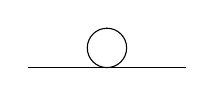
\begin{tikzpicture}[scale=1, transform shape]
		\draw (0,0) -- (2,0);
		\draw (1,0.25) circle[radius=0.25];
	\end{tikzpicture} 
	+
	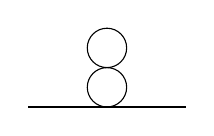
\begin{tikzpicture}[scale=1, transform shape]
		\draw (0,0) -- (2,0);
		\draw (1,0.25) circle[radius=0.25];
		\draw (1,0.75) circle[radius=0.25];
	\end{tikzpicture}
	+ 
	\begin{tikzpicture}[scale=1, transform shape,baseline=(a.base)]
		\draw (a) (0,0) -- (2,0);
		\draw (1,0) circle[radius=0.5];
	\end{tikzpicture}
	+ \dots \notag\\
	\shortintertext{Then the \underline{complete} propagator using $D^0_F(p^2) = \frac{i}{p^2 - m^2_0 +i\epsilon}$ is} 
	D_F(p^2) &= \int \dd^4 x e^{ipx} \braket{0 | T\phi(x)\phi(0) | 0} \\
			 &=
	\begin{tikzpicture}[scale=1, transform shape]
		\draw (0,0) -- (2,0);
	\end{tikzpicture} 
	+
	\begin{tikzpicture}[scale=1, transform shape,baseline=(a.base)]
		\draw (a) (0,0) -- (0.6,0);
		\draw (a) (1.4,0) -- (2,0);
		\draw (1,0) circle[radius=0.4];
		\node at (1,0) {$-i\Sigma$};
	\end{tikzpicture}
	+
	\begin{tikzpicture}[scale=1, transform shape,baseline=(a.base)]
		\draw (a) (-0.2,0) -- (0.2,0);
		\draw (0.6,0) circle[radius=0.4];
		\node at (0.6,0) {$-i\Sigma$};
		\draw (1,0) -- (1.2,0);
		\draw (1.6,0) circle[radius=0.4];
		\node at (1.6,0) {$-i\Sigma$};
		\draw (2,0) -- (2.4,0);
	\end{tikzpicture}  + \dots \notag\\
			 &= D^0_F(p^2) + D_F^0 (p^2) \left( -i\Sigma(p^2) \right)D^0_F(p^2)  + \dots \notag\\
	\shortintertext{it is cleary a geometric series}
			 &= \frac{D^0_F(p^2)}{1+i\Sigma(p^2)D_F^0(p^2)} \notag\\
			 &= \frac{i}{p^2 - m_0^2 -\Sigma(p^2)} \label{math:renormD}
\end{align}
The pole of propagator does not occur at $m_0^2$ anymore. It will be shifted by $\Sigma \sim \mathcal{O}(\lambda)$!

\paragraph{Expansion of divergent integrals}\footnote{see also Cheng and Li, Chapter 2.1}
Notice that the integral in \ref{math:M} $\propto \int \frac{\dd^4 q}{q^4}$. If we differentiate it with respect to $q$, the integral becomes convergent. This holds true for integral of general loop diagrams (although more than one differentiation might be needed). Thus we can expand this kind of integral into convergent and divergent term(s).

Expand
\begin{align}\label{math:Sigma}
	\Sigma(p^2) = \Sigma(m^2) + (p^2 - m^2) \Sigma'(m^2) + (p^2 - m^2)\tilde{\Sigma}(p^2)
\end{align}
where $\Sigma(m^2)$ is quadratically and $\Sigma'(m^2)$ logarithmically divergent.
$\tilde{\Sigma}$ represents a correction (to first order Taylor expansion) and it satisfies $\tilde{\Sigma}(m^2) = \tilde{\Sigma}'(m^2) = 0$.

\paragraph{Mass and field renormalization}
The mass $m$ by the condition 
\begin{align}
	m^2	= m_0^2 + \Sigma(m^2)
\end{align}
This is indeed physical mass, since the expression for propagator in \ref{math:renormD} has a pole at $p^2 = m^2$.

Then the propagator
\begin{align}
	D_F(p^2) =& \frac{i}{p^2 - m^2_0 - \Sigma(p^2)} = \frac{i}{p^2 - m^2 - (p^2 - m^2)(\Sigma '(m^2) + \tilde{\Sigma}(p^2))} \notag \\
	\shortintertext{using \ref{math:Sigma}}
	=& \frac{i}{(p^2 - m^2)(1-\Sigma'(m^2)-\tilde{\Sigma}(p^2))} \notag\\
	=& \frac{iZ}{p^2 - m^2} \cdot \frac{1}{1-Z\tilde{\Sigma}(p^2)} \notag \\
	=& \frac{iZ}{p^2 - m^2} + \text{(regular at $p^2 = m^2$)}
\end{align}
with $Z = \left( 1 - \Sigma '(m^2) \right)^{-1}$. This expression is to be compared with \ref{math:fourTwoP}.

Starting point Lagrangian is $\lag = \frac{1}{2}(\partial_\mu \phi_0)^2 - \frac{m^2_0}{2}\phi_0^2 - \frac{\lambda_0}{4!}\phi_0^4$. To remove $Z$ from numerator in the propagator and instead put $\sqrt{Z}$ onto the couplings at each end. Since each internal vertex has 4 lines (remember the vertex carries the coupling constant)
\begin{align}
	\lambda_0 \longmapsto \lambda_1 = Z^2 \lambda_0
\end{align}

In $\Sigma$ and $\tilde{\Sigma}$, there are 2 external lines without $\sqrt{Z}$, so
\begin{align}
	\Sigma(p^2, \lambda_0, \text{old } D_F) = \frac{1}{Z} \Sigma_1(p^2, \lambda_1, \text{new } D'_F)
\end{align}
(same expression for $\tilde{\Sigma}$).

Thus we get the new propagator
\begin{align}
	D'_F(p^2) = \frac{i}{p^2 - m^2} \cdot \frac{1}{1-\tilde{\Sigma}_1(p^2)}
\end{align}
where $\tilde{\Sigma}_1(m^2) = 0$.

Define the renomalized field
\begin{align}
	Z^{-\frac{1}{2}} \phi_0 = \phi
\end{align}
then $D'_F$ is the Fourier transform of $\braket{0 | T\phi(x)\phi(y) | 0}$

Rewrite the Lagrangian as
\begin{align}
	\lag = \frac{1}{2} \left( (\partial_\mu \phi)^2 - m^2 \phi^2 \right) \boxed{-\frac{\lambda_1}{4!}\phi^4 \underbrace{- \frac{1}{2}\delta m^2 \phi^2 + \frac{1}{2}(Z-1) \left( (\partial_\mu \phi)^2 - m^2 \phi^2 \right)}_{\text{counter-terms}} }
\end{align}
where $\delta m^2 = -Z(m^2 + m_0^2) = -Z\Sigma(m^2) = -\Sigma_1 (m^2)$. Everything inside the $\boxed{\text{box}}$ can be considered as interaction. 

It may look weird given the kinetic/mass-like terms, but there is no contradiction. Consider just $\lag = \frac{1}{2}(\partial \phi)^2 - \frac{m^2}{2}\phi^2$. The mass-term $\equiv$ "interaction".
A massless propagator $$\feynmandiagram[small, horizontal=a to b, baseline=(a.base)]{a--b}; = \frac{i}{p^2}$$ and interaction $$\feynmandiagram[small, horizontal=a to b, baseline=(a.base)]{a --[insertion=0.5] b;};=-im^2$$ The resummed propagator is then
\begin{align*}
	\feynmandiagram[layered layout, horizontal=a to x, small, baseline=(x.base)]{
		a -- x[blob] -- b;
	};
	=&
	\feynmandiagram[small, horizontal=a to b, baseline=(a.base)]{a --b;};
	+
	\feynmandiagram[small, horizontal=a to b, baseline=(a.base)]{a --[insertion=0.5] b;};
	+
	\feynmandiagram[small, horizontal=a to b, baseline=(a.base)]{a --[insertion=0.33, insertion=0.66] b;};
	+ \dots \\
	=& \frac{i}{p^2} \left( 1 + \frac{i}{p^2}(-im^2)+\dots \right) \\
	=& \frac{i}{p^2} \left( 1 - \frac{i}{p^2} (-im^2)\right)^{-1} = \frac{i}{p^2 - m^2} 
\end{align*}

Actually this is not all. We will also have to further renormalize $\lambda_1$
\begin{align*}
	\begin{tikzpicture}[scale=1, transform shape, baseline=(x.base)]
		\begin{feynman}
			\vertex (x1);
			\vertex (x2) at (2,0);
			\vertex (x3) at (0,-2);
			\vertex (x4) at (2,-2);
			\vertex (x) at (1,-1);
			\diagram*{
				(x1)-- (x) --(x2),
				(x3)-- (x) --(x4),
			};
		\end{feynman}
	\end{tikzpicture}
	+
		\begin{tikzpicture}[scale=1, transform shape, baseline=(x.base)]
		\begin{feynman}
			\vertex (x1);
			\vertex (x2) at (2,0);
			\vertex (x3) at (0,-2);
			\vertex (x4) at (2,-2);
			\vertex (xx) at (1,-0.6);
			\vertex (y) at (1,-1.4);
			\diagram*{
				(x1)-- (xx) --(x2),
				(x3)-- (y) --(x4),
				(xx) --[quarter left] (y) --[quarter left] (xx),
			};
		\end{feynman}
	\end{tikzpicture}
	+
	\begin{tikzpicture}[scale=1, transform shape, baseline=(x.base)]
		\begin{feynman}
			\vertex (x1);
			\vertex (x2) at (2,0);
			\vertex (x3) at (0,-2);
			\vertex (x4) at (2,-2);
			\vertex (x) at (0.6,-1);
			\vertex (y) at (1.4,-1);
			\diagram*{
				(x1)-- (x) --(x3),
				(x2)-- (y) --(x4),
				(x) --[quarter left] (y) --[quarter left] (x),
			};
		\end{feynman}
	\end{tikzpicture}
	+
	\begin{tikzpicture}[scale=1, transform shape, baseline=(x.base)]
		\draw (0,0) to  (0.6,-0.5) to[out=-45, in=45] (0.6, -1.5) to (0,-2);
		\draw (0.6, -0.5) to [out=180, in=-180] (0.6,-1.5);
		\draw (0.6, -0.5) to [out=0, in=90] (2, -2);
		\draw (0.6, -1.5) to [out=0, in=-90] (2,0);
	\end{tikzpicture}
	+ \dots = \lambda_1 \left\{ 1 + L + \Gamma(s,t,u) \right\}
\end{align*}

$L$ is value of the sum of all 1PI vertex contributions at the \underline{same} kinematic point and $\Gamma$ defined by $\Gamma(s=t=u=\frac{4}{3}M^2)=0$ (for instance, $P_i^2=M^2$ and $P_i P_j = -\frac{M^2}{3}$ with $i\neq j$).

Define 
\begin{align}
	Z_\lambda \defeq (1+L)^{-1}
\end{align}
and the renormalized coupling is
\begin{align}
	\lambda = Z_\lambda^{-1} \lambda_1 = Z_\lambda^{-1}Z^2 \lambda_0
\end{align}
Write Lagrangian in terms of renormalized $\lambda$ and add another counter-term $-\frac{(Z_\lambda-1)}{4!}\lambda \phi^4$.

Note that all counter-terms we have introduced are of the \underline{same form} as the original Lagrangian: $(\partial \phi)^2$, $\phi^2$ and $\phi^4$. There is no need to introduce new structure or new coupling parameters. It is property of a \underline{renormalizable theory}.

\section{Divergent graphs and dimensional regularization}
\begin{align*}
	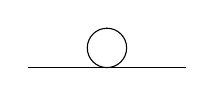
\begin{tikzpicture}[scale=1, transform shape]
	\draw (0,0) -- (2,0);
	\draw (1,0.25) circle[radius=0.25];
	\end{tikzpicture} 
\quad 
M_2 = \frac{\lambda}{2} \frac{1}{i} \int \frac{\dd^4 k}{(2\pi)^4} \frac{1}{k^2 - M^2 + i\epsilon}
\end{align*}
\begin{align*}	
\begin{tikzpicture}[scale=1, transform shape, baseline=(x.base)]
	\begin{feynman}
		\vertex (x1);
		\vertex (x2) at (2,0);
		\vertex (x3) at (0,-2);
		\vertex (x4) at (2,-2);
		\vertex (x) at (0.6,-1);
		\vertex (y) at (1.4,-1);
		\diagram*{
			(x1)-- (x) --(x3),
			(x2)-- (y) --(x4),
			(x) --[quarter left] (y) --[quarter left] (x),
		};
	\end{feynman}
\end{tikzpicture}
\quad
M_4 = \frac{\lambda^2}{2}\frac{1}{i}\int \frac{\dd^4 k}{(2\pi)^4} \frac{1}{(k^2 - M^2 +i\epsilon)((k-p)^2-M^2+i\epsilon)}
\end{align*}

\paragraph{Wick rotation}
Poles of $M_2$ in the complex $k^0$-plane at $k^0 = \pm \sqrt{\pmb{k}^2 + M^2 - i\epsilon}$. The position of the poles allow us to \underline{rotate} the integration path to go $-i\infty \mapsto +i\infty$ instead. So no singularities are hit!

\begin{center}
\begin{tikzpicture}[scale=1, transform shape]
	\draw[->] (-2,0) -- (2,0);	
	\draw[->] (0,-2) -- (0,2);
	\node [below] at (2,0) {$\Re(k^0)$};
	\node [left] at (0,2) {$\Im(k^0)$};
	\draw[->, thick, blue] (-1.7,0) -- (-0.5,0);
	\draw[->, thick, blue] (-0.5,0) -- (1,0);
	\draw[thick, blue] (1,0) -- (1.7,0);
	\draw[->, thick, red] (0,-1.7) -- (0,-0.5);
	\draw[->, thick, red] (0,-0.5) -- (0,1);
	\draw[thick, red] (0,1) -- (0,1.7);
	\draw[->,red, dashed] (1.5,0) to [out=90, in=0] (0,1.5);
	\draw[->,red, dashed] (-1.5,0) to [out=-90, in=-180] (0,-1.5);
\end{tikzpicture}
\end{center}

Define a Euclidean momentum $k^0 = ik_E^0$, $\pmb{k} = \pmb{k}_E$
\begin{align*}
	\frac{1}{i}\int \frac{\dd k^0 \dd^3 k}{(2\pi)^4} \frac{1}{(k_0)^2 - \pmb{k}^2 - M^2 +i\epsilon} \longmapsto - \int \frac{\dd^4 k_E}{(2\pi)^4} \frac{1}{k^2_E + M^2 -i\epsilon}
\end{align*}
Now we are far from singularities, $i\epsilon$ can thus be ignored.

This form allows us to see
\begin{itemize}[label={}]
	\item 
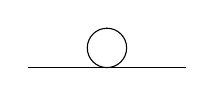
\begin{tikzpicture}[scale=1, transform shape]
	\draw (0,0) -- (2,0);
	\draw (1,0.25) circle[radius=0.25];
\end{tikzpicture} 
$\sim \int \frac{\dd k k^3}{k^2}$ is quadratically divergent

\item
\begin{tikzpicture}[scale=1, transform shape, baseline=(x.base)]
	\begin{feynman}
		\vertex (x1);
		\vertex (x2) at (2,0);
		\vertex (x3) at (0,-2);
		\vertex (x4) at (2,-2);
		\vertex (x) at (0.6,-1);
		\vertex (y) at (1.4,-1);
		\diagram*{
			(x1)-- (x) --(x3),
			(x2)-- (y) --(x4),
			(x) --[quarter left] (y) --[quarter left] (x),
		};
	\end{feynman}
\end{tikzpicture}
$\sim \int \frac{\dd k k^3}{k^4}$ is logarithmically divergent
\end{itemize}

Hope of renormalization program is that all such divergences can be absorbed into bare/unrenormalized couplings to produce physical/renormalized/observable parameters.

There are different methods to regularize divergent loop integrals in order to keep track of divergences
\begin{enumerate}
	\item momentum ($\Lambda$) cutoff: study the limit $\Lambda \longmapsto \infty$ in the end
	\item Pauli-Villars: subtract propagator(s) with heavy mass(es)\footnote{for details see Ryder, Chapter 9.2}
		\begin{align*}
			\frac{1}{k^2} \longmapsto \frac{1}{k^2} - \frac{1}{k^2 - M^2_\text{PV}}, M_\text{PV} \longmapsto \infty
		\end{align*}
	\item dimensional regularization: work in $d$ dimension instead of $4$, $1$ time-like, $d-1$ space-like. For small $d$ integral converge, consider $d \longmapsto 4$ in the end. The divergences appear as poles in $\frac{1}{d-4}$.
\end{enumerate}
Main advantage of dimensional regularization is that all symmetries are preserved (massless photons etc.). Downside is that it is somewhat unphysical and unintuitive.

\paragraph{Feynman parameters}\footnote{see also Peskin and Schröder, Chapter 6.3; Ryder, Chapter 9.2} Combine multiple propagators into one (to some power)
\begin{align}
	\frac{1}{A_1 \dots A_n} = \int^1_0 \dd x_1 \dots \dd x_n \delta \left(\sum_i^n x_i - 1 \right) \frac{(n-1)!}{(x_1 A_1 + \dots + x_n A_n)^n}
\end{align}
using 
\begin{align*}
	\frac{1}{A_i} &= \int^\infty_0 \dd \alpha_i e^{-\alpha_i A_i} \\
	\int \dd \alpha_1 \dots \dd \alpha_n e^{-\sum_i \alpha_i A_i} &= \int^1_0 \dd x_1 \dots \dd x_n \delta \left(\sum^n_i x_i - 1\right) \int^\infty_0 \dd t\; t^{n-1} e^{-t\sum_i x_i A_i}
\end{align*}

Special case
\begin{align}
	\frac{1}{AB} = \int^1_0 \dd x \frac{1}{ \left[ xA + (1-x)B \right]^2  }
\end{align}

With $A = (k-p)^2 - M^2$ and $B=k^2-M^2$
 \begin{align*}
	xA+(1-x)B = k^2 - xp(2k-p) - M^2 = (k-p)^2 - (M^2 -x(1-x)p^2)
\end{align*}

Thus after shifting the integration variable $k \longmapsto k+xp$ and with $\Delta(x) \defeq M^2 - x(1-x)p^2$
\begin{align*}
	\int \frac{\dd^d k}{(2\pi)^d} \frac{1}{(k^2-M^2)((k-p)^2-M^2)} = \int^1_0 \dd x \int \frac{\dd^d k}{(2\pi)^d} \frac{1}{[k^2 - \Delta(x)]^2}
\end{align*}

\paragraph{Dimensional regularization formula}\footnote{see also Peskin and Schröder, Chapter 7.5}
\begin{align}
	\frac{1}{i} \int \frac{\dd^d k}{(2\pi)^d} \frac{1}{(k^2 - \Delta)^n} = \frac{(-1)^n}{(4\pi)^{d/2}} \frac{\Gamma(n-d/2)}{\Gamma(n)} \frac{1}{\Delta^{n-d/2}}
\end{align}
$\Gamma$-function has following definition and properties
\begin{itemize}
	\item $\Gamma(n+1) = \int^\infty_0 \dd x x^n e^{-x}$
	\item $\Gamma(n+1) = n!$ for $n \in \N$, $n\Gamma(n) = \Gamma(n+1)$
	\item $\Gamma(n)$ has poles for negative integers $n=0, -1, -2, \dots$
\end{itemize}

\paragraph{Proof by induction}
\begin{itemize}
\item $n=1$: introduce \underline{Schwinger parameter} $\alpha$ and $i\epsilon$ part enforces convergence.
\begin{align*}
	\frac{1}{i} \int \frac{\dd^d k}{(2\pi)^d} \frac{1}{k^2 - \Delta + i\epsilon} 
	&= -\int^\infty_0 \dd \alpha \int \frac{\dd^d k}{(2\pi)^d} e^{i\alpha (k^2 - \Delta + i\epsilon)} \\
	\shortintertext{using Wick rotation}
	&= -i\int^\infty_0 \dd \alpha \int \frac{\dd^d k_E}{(2\pi)^d}e^{-i\alpha (k_E^2 + \Delta - i\epsilon)}\\
	\shortintertext{Gaussian integral in higher dimension; in general $ \int \exp\left( - \frac 1 2 x \cdot A \cdot x +J \cdot x \right) d^nx = \sqrt{\frac{(2\pi)^n}{\det A}} \exp \left( {1\over 2} J \cdot A^{-1} \cdot J \right)$}
	&= \frac{-i}{(2\pi)^d} \int^\infty_0 \dd \alpha {\sqrt{\frac{\pi}{i\alpha}}}^d e^{-i\alpha \Delta} \\
	&= \frac{-i}{(4\pi)^{d/2}} \int^\infty_0 \dd \alpha (i\alpha)^{-d/2} e^{-i\alpha \Delta} \\
	&= -\frac{1}{(4\pi)^{d/2}} \frac{1}{\Delta^{1-d/2}} \int^\infty_0 \dd x x^{-d/2} e^{-x} \\
	&= \frac{(-1)}{(4\pi)^{d/2}}\frac{1}{\Delta^{1-d/2}} \Gamma(1-d/2)
\end{align*}
\item Induction $n \rightarrow n+1$
	\begin{align*}
		\frac{1}{i} \int \frac{\dd^d k}{(2\pi)^d} \frac{1}{(k^2-\Delta)^{n+1}}
		&= \frac{1}{n} \frac{\partial}{\partial \Delta} \frac{1}{i} \int \frac{\dd^d k}{(2\pi)^d} \frac{1}{(k^2-\Delta)^n} \\
		&= \frac{1}{n} \frac{\partial}{\partial \Delta} \left( \frac{(-1)^n}{(4\pi)^{d/2}} \frac{\Gamma(n-d/2)}{\Gamma(n)} \frac{1}{\Delta^{n-d/2}} \right) \\
		&= \frac{(-1)^{n+1}}{(4\pi)^{d/2}} \frac{\Gamma(n-d/2)}{n\Gamma(n)} \left( n-\frac d 2 \right)  \frac{1}{\Delta^{n+1-d/2}} \\
		&= \frac{(-1)^{n+1}}{(4\pi)^{d/2}} \frac{\Gamma(n+1-d/2)}{\Gamma(n+1)} \frac{1}{\Delta^{n+1-d/2}} \qquad \square
	\end{align*}
\end{itemize}

There is another change in $d$ dimensions. Since $S=\int\dd^d x \lag$ is dimensionless (keep in mind we are working in natural units), $[\lag] = M^d$. So $\lag_{\text{KG}} = \frac{1}{2}(\partial_\mu \phi)^2 - \frac{M^2}{2}\phi^2$ suggests now $[\phi]=M^{d/2-1}$ and in Dirac theory $[\psi] = M^{\frac{d-1}{2}}$. So in order to keep $[\lambda] = M^0 = 1$, $\lag_{\phi^4}=-\mu^{4-d} \frac{\lambda}{4!} \phi^4$ with $\mu$ an arbitrary mass parameter $[\mu] = M^1$.

With dimensional regularization 
\begin{align*}
	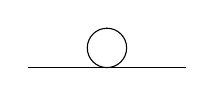
\begin{tikzpicture}[scale=1, transform shape]
		\draw (0,0) -- (2,0);
		\draw (1,0.25) circle[radius=0.25];
	\end{tikzpicture} 
	&= \frac{\mu^{4-d}\lambda}{2} \frac{1}{i} \int \frac{\dd^d k}{(2\pi)^d} \frac{1}{k^2 - M^2 + i\epsilon} \\
	&= \frac{\lambda}{2} \mu^{4-d} \left( -\frac{1}{(4\pi)^{d/2}} \right) M^{d-2}\Gamma(1-d/2) \\
	&\boxed{
		\begin{array}{ll}
			&\text{Laurent expansion} \\
			 \Gamma(z) &= \frac{1}{z} - \gamma_E + \mathcal{O}(z), \quad  z\rightarrow 0\\
			\Gamma(z-1) &= \frac{1}{z-1} \Gamma(z), \quad z\rightarrow 0\\
						&= -\left( 1+z+\mathcal{O}(z^2) \right) \Gamma(z) \\
						&= -\frac{1}{z} + \gamma_E - 1 + \mathcal{O}(z) \\
			\gamma_E &= 0.5772\dots
		\end{array}
	}\\
	&= -\frac{\lambda}{2} 	\frac{M^2}{8\pi^2} \left( \frac{M^2}{4\pi\mu^2} \right)^{\frac{d-4}{2}} \left[ \frac{1}{d-4} + \frac{1}{2}(\gamma_E - 1) + \mathcal{O}(d-4) \right] \\
	\shortintertext{Taylor expansion around $\epsilon=0$, $a^\epsilon = 1 + \epsilon \ln{a}$}
	&= -\frac{\lambda}{2} 	\frac{M^2}{8\pi^2} \left\{ \frac{1}{d-4} + \frac 1 2 \left[ \gamma_E - 1 - \ln(4\pi) \right] + \ln{\frac{M}{\mu}}  + \mathcal{O}(d-4) \right\}
\end{align*}

\begin{align*}
	\shortintertext{with $\Delta(x) = M^2 - x(1-x)p^2$}
	\begin{tikzpicture}[scale=1, transform shape, baseline=(x.base)]
	\begin{feynman}
		\vertex (x1);
		\vertex (x2) at (2,0);
		\vertex (x3) at (0,-2);
		\vertex (x4) at (2,-2);
		\vertex (x) at (0.6,-1);
		\vertex (y) at (1.4,-1);
		\diagram*{
			(x1)-- (x) --(x3),
			(x2)-- (y) --(x4),
			(x) --[quarter left] (y) --[quarter left] (x),
		};
	\end{feynman}
	\end{tikzpicture}
	&= \frac{\mu^{2(4-d)} \lambda^2}{2} \frac{1}{i} \int_0^1 \dd x \int \frac{\dd^d k}{(2\pi)^d} \frac{1}{[k^2 - \Delta(x)]^2} \\
	&= \frac{\lambda^2}{2} \mu^{2(4-d)} \int^1_0 \dd x \frac{1}{(4\pi)^{d/2}}\frac{\Gamma(2-d/2)}{2} \frac{1}{\Delta(x)^{2-d/2}} \\
	&= \frac{\lambda^2}{2} \frac{\mu^{4-d}}{(4\pi)^2} \left\{ -2 \left[ \frac{1}{d-4} + \frac{1}{2}(\gamma_E - \ln{4\pi}) + \ln(\frac{M}{\mu}) \right] - \int^1_0 \dd x \ln(\frac{\Delta(x)}{M^2}) \right\}\\
%%%%%%%%%%%%%%%%%%%%%%%%%%%%%%%%%%%%%%%%%%%
	\int^1_0 \dd x \ln(\frac{\Delta(x)}{M^2})&=\int_0^1 \dd x \ln{\frac{M^2-x(1-x)p^2}{M^2}}  \\
											 &= \int_0^1 \dd x \ln{ \left[ \left(\frac{\sigma+1}{2} - x \right)\left(x+\frac{\sigma-1}{2}\right) \right] } - \ln{\frac{\sigma^2 - 1}{4}} , \quad \sigma = \sqrt{1-\frac{4M^2}{p^2}} \\
	&= \sigma \ln{\frac{\sigma+1}{\sigma-1}} - 2
\end{align*}
Valid for $p^2 < 0$, rest by analytic continuation

Compare $M(s) - M(0)$ calculated based on Cutkosky and dispersion integral. Easier 
\begin{align*}
	M(0) &= \frac{1}{i} \int \frac{\dd^d k}{(2\pi)^d} \frac{1}{(k^2 - M^2)^2} \\
		 &= \frac{\partial}{\partial M^2} \frac{1}{i} \int \frac{\dd^d k}{(2\pi)^d} \frac{1}{k^2 - M^2} \\
		 &= \frac{\partial}{\partial M^2} \left\{ -\frac{M^2}{8\pi^2} \left[ \frac{1}{d-4} + \frac{1}{2}(\gamma_E - 1 -\ln{4\pi}) + \frac{1}{2} \ln{\frac{M^2}{\mu^2}} \right] \right\} \\
	\shortintertext{$1$ gets cancalled by the derivative of $\ln$}
		 &= - \frac{1}{8\pi^2} \left[ \frac{1}{d-4} + \frac{1}{2} \left(\gamma_E - \ln{4\pi} + \frac{1}{2} \ln{\frac{M^2}{\mu^2}}\right) \right]
\end{align*}

Lets summarise the renormalization of $\phi^4$ at one loop
\begin{itemize}
	\item
	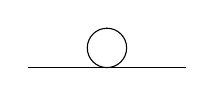
\begin{tikzpicture}[scale=1, transform shape]
		\draw (0,0) -- (2,0);
		\draw (1,0.25) circle[radius=0.25];
	\end{tikzpicture} 
		is \underline{independent} of $p^2$! Hence $\Sigma(p^2)$ at $\mathcal{O}(\lambda)$ only renormalises the \underline{mass}, there is no wave-function renormalization $Z (\sim \frac{\partial \Sigma}{\partial p^2} |_{p^2 = M^2}) \quad \rightarrow Z=1 + \mathcal{O}(\lambda^2)$ \\
		This does change at $\mathcal{O}(\lambda^2)$ 
	\feynmandiagram[layered layout, small, horizontal=a to b, baseline=(a.base)]{
	a -- x;
	x --[half left] y;
	x --[half right] y;
	x -- y;
	y -- b;
	};	
$\rightarrow Z\neq 1$
\item Mass renormalization
	\begin{align*}
		\feynmandiagram[layered layout, horizontal=a to x, small, baseline=(x.base)]{
			a -- x[blob, label=\(-iM^2\)] -- b;
		}; 
		&=
		\feynmandiagram[layered layout, horizontal=a to x, small, baseline=(x.base)]{
			a -- x[blob, label=\(-iM^2\)] -- b;
		};
		+
		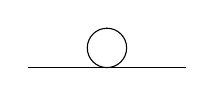
\begin{tikzpicture}[scale=1, transform shape]
			\draw (0,0) -- (2,0);
			\draw (1,0.25) circle[radius=0.25];
		\end{tikzpicture} 
		+
		\feynmandiagram[layered layout, horizontal=a to x, small, baseline=(x.base)]{
			a -- x[blob, label=\(-i\delta M^2\)] -- b;
		};
		\\ 
		\delta M^2 &= M_0^2 - M^2
		\shortintertext{then}
		M^2 &= M^2 + \frac{\lambda M^2}{16\pi^2} \left[ \frac{1}{d-4} + \frac{1}{2} \left(\gamma_E - 1 -\log{4\pi} + \log{\frac{M}{\mu}}\right) \right]- M^2 + M_0^2 \\
		\delta M^2	&= \frac{\lambda M^2}{16\pi^2} \left[ \frac{1}{d-4}  + \frac{1}{2} \left(\gamma_E - 1 - \log{4\pi} + \log{\frac{M}{\mu}} \right) + \mathcal{O}(\lambda, (d-4)) \right] \\
	\end{align*}
	Physical mass $M^2_\text{phy}$ cannot be dependent on $\mu$, meaning $\lambda \mu^{4-d} M^2 = \lambda_0 M_0^2 + \mathcal{O}(\lambda^2)$ and $\lambda_0$ and $M_0$ are independent of $\mu$.
	\item Coupling constant renormalization. Lets choose renormalization point for $\lambda$ at $s=t=u=0$ for simplicity:
\begin{align*}
	\feynmandiagram[small, baseline=(x.base),layered layout]{
		x1 -- x[blob] -- x2;
		x3 -- x -- x4;
	};
	&=
	\begin{tikzpicture}[scale=1, transform shape, baseline=(x.base)]
	\begin{feynman}
		\node (x1) ;
		\node (x2) at (2,0);
		\node (x3) at (0,-2);
		\node (x4) at (2,-2);
		\vertex (x)[dot] at (1,-1);
		\diagram*{
			(x1)-- (x) --(x2),
			(x3)-- (x) --(x4),
		};
	\end{feynman}
\end{tikzpicture}
+
	\begin{tikzpicture}[scale=1, transform shape, baseline=(x.base)]
	\begin{feynman}
		\node (x1);
		\node (x2) at (2,0);
		\node (x3) at (0,-2);
		\node (x4) at (2,-2);
		\vertex (xx) at (1,-0.6);
		\vertex (y) at (1,-1.4);
		\diagram*{
			(x1)-- (xx) --(x2),
			(x3)-- (y) --(x4),
			(xx) --[quarter left] (y) --[quarter left] (xx),
		};
	\end{feynman}
\end{tikzpicture}
+
\begin{tikzpicture}[scale=1, transform shape, baseline=(x.base)]
	\begin{feynman}
		\node (x1);
		\node (x2) at (2,0);
		\node (x3) at (0,-2);
		\node (x4) at (2,-2);
		\vertex (x) at (0.6,-1);
		\vertex (y) at (1.4,-1);
		\diagram*{
			(x1)-- (x) --(x3),
			(x2)-- (y) --(x4),
			(x) --[quarter left] (y) --[quarter left] (x),
		};
	\end{feynman}
\end{tikzpicture}
+
\begin{tikzpicture}[scale=1, transform shape, baseline=(x.base)]
	\begin{feynman}
		\node (x2) at (0,0);
		\node (x1) at (2,0);
		\node (x3) at (0,-2);
		\node (x4) at (2,-2);
		\vertex (x) at (0.6,-1);
		\vertex (y) at (1.4,-1);
		\diagram*{
			(x1)--[quarter right] (x) --(x3),
			(x2)--[quarter left] (y) --(x4),
			(x) --[quarter left] (y) --[quarter left] (x),
		};
	\end{feynman}
\end{tikzpicture}
+
	\feynmandiagram[small, baseline=(x.base),layered layout]{
		x1 -- x[crossed dot] -- x2;
		x3 -- x -- x4;
	}; \\
	&= 
	 -i\lambda\mu^{4-d} 
	+ i\left(M(s) + M(t) + M(u)\right)
	- i(Z_\lambda-1)\lambda\mu^{4-d} 
	+ \mathcal{O}(\lambda^3)\\
	\shortintertext{with $Z=1$}
			\lambda_0 &=  \lambda \mu^{4-d}Z_\lambda = \lambda \mu^{4-d} \bigg\{ \underbrace{ 1- \frac{3}{\lambda}{16\pi^2} \bigg[ \frac{1}{d-4} }_{Z^{MS}_\lambda \text{ minimal subtraction}} +\frac{1}{2} \bigg(\gamma_E -\log{4\pi} + \log{\frac{M}{\mu}} \bigg) \bigg] + \mathcal{O}(\lambda^2) \bigg\} \\
			&=  \lambda \mu^{4-d}Z_\lambda = \lambda \mu^{4-d} \bigg\{ \underbrace{1- \frac{3}{\lambda}{16\pi^2} \bigg[ \frac{1}{d-4} +\frac{1}{2} \bigg(\gamma_E -\log{4\pi} }_{Z^{\bar{MS}}_\lambda \text{modified minimal subtraction}} + \log{\frac{M}{\mu}}\bigg)\bigg] + \mathcal{O}(\lambda^2) \bigg\} \\
			\shortintertext{\text{these two $Z$ are mass-indepent}}
			&=  \lambda \mu^{4-d}Z_\lambda = \lambda \mu^{4-d} \bigg\{ \underbrace{1- \frac{3}{\lambda}{16\pi^2} \bigg[ \frac{1}{d-4} +\frac{1}{2} \bigg(\gamma_E -\log{4\pi}  + \log{\frac{M}{\mu}}\bigg)\bigg] }_{Z_\lambda \text{mass-dependent}}+ \mathcal{O}(\lambda^2) \bigg\} 
		\end{align*}
\end{itemize}

\section{Superficial degree of divergence}
How do we know that we are done renormalising the theory with
\begin{itemize}
	\item wave function
	\item mass
	\item coupling
\end{itemize}
Can't there be more divergences?

Want to analyse superficial degree of divergence $D$ of an arbitrary loop diagram with 
\begin{itemize}
	\item $d$ dimension
	\item $L$ number of loops
	\item $I$ number of internal propagators
	\item $E$ number of external lines
	\item $V$ number of vertices
\end{itemize}

Matrix element of an arbitrary diagram generically 
\begin{align*}
	\sim \lambda^V \int \frac{\dd^d k_1 \dd^d k_2 \dots \dd^d k_L}{(k_{i_1}^2 - M^2) \dots (k_{i_I}^2 - M^2)}
\end{align*}
So clearly 
\begin{align}
	D = d L - 2 I
\end{align}

$D \geq 0 $ divergent ($D=0$ logarithmically divergent) and $D < 0$ convergent.

Express $L$ and $I$ in terms of $V$ and $E$
\begin{align}
	L &= \text{number of undetermined integration momenta} \notag \\
	  &= \text{number of internal propagators} - \text{number of momentum conservations at vertices} \notag\\
	  &\quad+ 1 \text{ (because of overall momentum conservation)} \notag \\
	L &= I - V + 1 \label{math:super1}
\end{align}
One vertex is linked to 4 legs. Internal lines are attached to 2 vertices and external line to 1.
\begin{align}
	4V = 2I + E \label{math:super2}
\end{align}
solve \ref{math:super1} and \ref{math:super2} for $L$ and $I$
\begin{align}
	D &= d + (d-4) V - \left(\frac{d}{2} - 1\right)E \\
	\shortintertext{in physical 4 dimension}
	D &= 4 - E
\end{align}

\paragraph{Remarks}
\begin{itemize}
	\item for $d=4$, $D$ is \underline{independent} of $V$, only dependent on $E$.
	\item only a few small $E$ produce $D \geq 0$, here in $\phi^4$
		$$E = 2 \quad \feynmandiagram[small, layered layout, inline=(x.base),horizontal=a to x]{a -- x[blob] -- b};$$
		$$E = 4 \quad \feynmandiagram[small, layered layout, inline=(x.base)]{a -- x[blob] -- b, c -- x -- d};$$
	\item distinguish theories of different $d$
		\begin{itemize}
			\item $d < 4$: $D$ \underline{decreases} with $V$, only finite number of diagrams (not n-point functions) diverges.
				\textbf{super-renormalizable}
			\item $d=4$: $D$ is \underline{independent} of $V$, only a finite number of amplitudes diverges, but at each order in perturbation theory.
				\textbf{renormalizable}
         \item $d>4$: $D$ \underline{grows} with $V$, even amplitude becomes divergent at some order in perturbation theory.
				\textbf{non-renormalizable}
		\end{itemize}
	\item alternative characterisation in terms of \underline{mass dimension} of coupling constant
		\begin{align*}
			\lag_{\phi^4} = -\mu^{4-d}\frac{\lambda}{4!} \phi^4 = - \frac{\tilde{\lambda}}{4!} \phi^4
		\end{align*}
		so $[\tilde{\lambda}] = 4-d$ in $d$ dimension; hence 
			\begin{itemize}
				\item $[\tilde{\lambda}] > 0$ super-renormalizable
				\item $[\tilde{\lambda}] = 0$ renormalizable
				\item $[\tilde{\lambda}] < 0$ non-renormalizable
			\end{itemize}
		\item why is this "superficial"? There can always be divergent sub-graphs! These sub-graphs are regularised and renormalised by the treatment of the "primitive divergences" we have already seen before.
\end{itemize}
\paragraph{Conclusion for $\phi^4$}
the only primitive divergences are $E=2$ and $E=4$ (and $E=0$ the vacuum graphs) and we renormalise the theory by  
\begin{align*}
	M_0^2 &= M^2 \left\{ 1 + c_m^{(1)}\frac{\lambda}{d-4} + c_m^{(2)}\frac{\lambda^2}{(d-4)^2} + \dots \right\} \\
	\lambda_0 &= \lambda \left\{ 1 + c_\lambda^{(1)}\frac{\lambda}{d-4} + c_\lambda^{(2)}\frac{\lambda^2}{(d-4)^2} + \dots \right\} \\
	Z &= 1 + c_z^{(2)} \frac{\lambda^2}{(d-4)^2} + \dots
\end{align*}

\section{Sketch of renormalization of QED}
Superficial degree of divergence with $E_\gamma$ external photons and $E_e$ external electrons.
\begin{align}
	D &= d + V \left(\frac{d-4}{2} \right) - E_e \left( \frac{d-1}{2} \right) - E_\gamma \left( \frac{d-2}{2} \right)\notag\\
	  &= 4 - \frac{3}{2}E_e - E_\gamma 
\end{align}
Again the superficial degree of divergence $D$ is independent of $V$, i.e. QED is renormalizable ($e$ is dimensionless as well).

We have following divergent diagrams
\begin{enumerate}[label=(\alph*)]
	\item \label{item:a} $\begin{aligned}[t]\feynmandiagram[small]{a[blob];}; \quad D &=4 \end{aligned}$
   \item \label{item:b} $\begin{aligned}[t]\feynmandiagram[small, horizontal=a to b, inline=(b.base)]{a[blob] --[photon] b;}; \quad D &=3\end{aligned}$
	\item \label{item:c}$\begin{aligned}[t]\feynmandiagram[small, horizontal=a to b, layered layout, inline=(b.base)]{a --[photon] b[blob] --[photon] c;}; \quad D &=2\end{aligned}$
	\item \label{item:d}$\begin{aligned}[t]\feynmandiagram[small, horizontal=a to c, spring layout, inline=(b.base)]{a --[photon] b[blob] --[photon] c; d --[photon] b;}; \quad D &=1\end{aligned}$
   \item \label{item:e}$\begin{aligned}[t]\feynmandiagram[small, horizontal=a to c, layered layout, inline=(b.base)]{a --[photon] b[blob] --[photon] c; d --[photon] b --[photon] e;}; \quad D &=0\end{aligned}$
	\item \label{item:f}$\begin{aligned}[t]\feynmandiagram[small, horizontal=a to b, layered layout, inline=(b.base)]{a --[fermion] b[blob] --[fermion] c;}; \quad D &=1\end{aligned}$
	\item \label{item:g}$\begin{aligned}[t]\feynmandiagram[small, horizontal=a to c, spring layout, inline=(b.base)]{a --[fermion] b[blob] --[fermion] c; d --[photon] b;}; \quad D &=1\end{aligned}$
\end{enumerate}

Still need to show that all divergences can be absorbed in the renormalization of the parameters of the theory.
\begin{align*}
	e_0 &\longmapsto e \\
	m_0 &\longmapsto m \\
	\psi &\longmapsto Z^{-1/2}_2 \psi \\
	A_\mu &\longmapsto Z^{-1/2}_3 A_\mu \\
	Z_1 &\equiv \text{ vertex correction (diagram (g) as $Z_\lambda$ in $\phi^4$)} 
\end{align*}

We now focus on individual divergent graphs. Diagram \ref{item:a}, vacuum diagram, is to be ignored. Diagrams \ref{item:b} and \ref{item:d} are not possible, since QED is $\mathcal{C}$-invariant, $A_\mu \longmapsto -A_\mu$. It can be generalized into Furry's theorem: correlation functions of odd number of photons vanish. Diagram \ref{item:e} is worrisome! Divergence would require counter-terms $\sim (F_{\mu\nu}F^{\mu\nu})^2, (F_{\mu\nu}\tilde{F}^{\mu\nu})^2$, dimension 8 operator. $[g_{A^4}] = M^{-4}$, i.e.~non-renormalizable! Here gauge-invariance is to rescue.

\begin{align*}
	\begin{tikzpicture}[scale=1, transform shape, baseline=(a.base)]
		\begin{feynman}
			\vertex (a);
			\vertex [right=of a] (b);
			\vertex [above=of a](c);
			\vertex [above=of b](d);
			\node [below left=of a] (q1) {\(q_1, \mu\)};
			\node [below right=of b](q2) {\(q_2, \nu\)};
			\node [above left=of c](q3) {\(q_3, \lambda\)};
			\node [above right=of d](q4) {\(q_4, \rho\)};
		\diagram*{
			(q1) --[photon] (a);
			(q2) --[photon] (b);
			(q3) --[photon] (c);
			(q4) --[photon] (d);
			(a) --[fermion, edge label'={$q_1 + k$}] (b) --[fermion, edge label'=\(q_1+q_2+k\)] (d) --[fermion,edge label'=\(q_3 + k\)] (c) --[fermion, edge label'=\(k\)] (a);
		};
		\end{feynman};
	\end{tikzpicture}
	&= \frac{e^4}{i} \int \frac{\dd^d k}{(2\pi)^4} \frac{\gamma_\mu (\slashed{k}+m) \gamma_\lambda (\slashed{q}_3 + \slashed{k} + m) \gamma_\rho (\slashed{q}_1 + \slashed{q}_2 + \slashed{k}+m) \gamma_\nu (\slashed{q}_1 + \slashed{k} + m)}{(k^2 - m^2) [(q_3 + k)^2 - m^2] [(q_1 + q_2 + k)^2 - m^2][(q_1+k)^2-m^2]} \\
	&= \frac{e^4}{i} \int \frac{\dd^4 k}{(2\pi)^4} \frac{\gamma_\mu \slashed{k} \gamma_\lambda \slashed{k} \gamma_\rho \slashed{k} \gamma_\nu \slashed{k}}{k^8} + \text{convergent terms}	 \\
   &= e^4 I(g_{\mu\lambda} g_{\rho\nu} + g_{\mu\rho}g_{\lambda\nu} + g_{\mu\nu}g_{\lambda\rho}) + \text{ finite }
   \shortintertext{because of Ward Identity $q_1^\mu (\dots) = 0$}
   &= I(q_{1\lambda}g_{\rho\nu}+q_{1\rho}g_{\lambda\nu}+q_{1\nu}g_{\lambda\rho}) + \text{ finite } = 0
   \shortintertext{thus digram \ref{item:e} is finite.}
\end{align*}
As a result the only primitively divergent graphs are diagram \ref{item:c} photon self energy, \ref{item:f} electron self energy, \ref{item:g} vertex graph!

We will discuss these in detail next term. The results at one loop are
\begin{align*}
   & \feynmandiagram[layered layout, small, horizontal=a to b]{a[particle=\(p\)] --[fermion] b -- c --[fermion] d; b--[half left, photon]c;}; &&= -i\Sigma(p) = \frac{-ie^2}{8\pi^2 (d-4)} (\slashed{p}-4m) + \text{finite} \\
   & \feynmandiagram[layered layout, small, horizontal=a to b, baseline=(a.base)]{a[label=\(k\)] --[photon] b --[opacity=0] c --[photon] d; b--[half left, anti fermion]c;b--[half right, fermion]c;}; &&= -i\Pi_{\mu\nu}(k) = \frac{ie^2}{6\pi^2 (d-4)} (g_{\mu\nu} k^2 - k_\mu k_\nu) \left[ \frac{1}{d-4} + (\text{finite, const.}) - \frac{k^2}{10m^2} + \dots \right] \\
   & \begin{tikzpicture}[scale=1, baseline=(c.base)]
      \begin{feynman}
         \node (a) at (0,0) {$p$};
         \vertex (b) at (1,0);
         \vertex (c) at (2,0);
         \vertex (d) at (3,0);
         \node (e) at (4,0) {$p'$};
         \node (x) at (2,1) {$q$};
         \diagram*{
         (a) --[fermion] (b) -- (c) -- (d) --[fermion] (e);
         (x) --[photon] (c);
         (b) --[half right, photon] (d);
         };
      \end{feynman};
   \end{tikzpicture} &&= ie\mu^{2-d/2}\Lambda_\mu;  \quad \Lambda_\mu = \frac{-e^2}{8\pi^2(d-4)} \gamma_\mu + \text{ finite }
   \shortintertext{"finite" contains $\frac{\alpha}{2\pi} \frac{i\sigma_{\mu\nu} q^\nu}{2m}$ anomolous magnetic moment}
\end{align*}

We have three renormalization factors
\begin{itemize}
   \item vertex 
      \begin{align}
         Z_1 = 1 + \frac{e^2}{8\pi^2(d-4)}
      \end{align}
   \item electron wave-function 
         \begin{align}
            Z_2 = 1 +\frac{e^2}{8\pi^2(d-4)}
         \end{align}
   \item photon wave-function 
      \begin{align}
         Z_3 = 1 + \frac{e^2}{6\pi^2(d-4)}
      \end{align}
\end{itemize}

Mass renormalization 
\begin{align}
   m_0 = Z^{-1}_2 (m+\delta m) = m \left( 1 + \frac{3e^2}{8\pi^2(d-4)} \right)
\end{align}

Coupling renormalization
\begin{align}
   e_0 = \mu^{2-d/2}Z_1 Z_2^{-1} Z_3^{-1/2} e = \mu^{2-d/2} Z_3^{-1/2} e
\end{align}

\paragraph{Remarks}
\begin{itemize}
   \item $Z_1 = Z_2$ is a fundamental consequence of the Ward Identity (consequence of gauge-invariance)
      \begin{align*}
      \begin{tikzpicture}[baseline=(m.base)]
      \begin{feynman}
         \node (a) at (0,0);
         \vertex (b) at (0, -1);
         \vertex (c) at (0, -2);
         \node (d) at (0,-3);
         \vertex (x) at (0.5, -1.5);
         \node (y) at (1.5, -1.5);
         \vertex (z) at (-0.5, -1.5);
         \node (m) at (0, -1.5) {\(\Gamma_\mu\)};
         \diagram*{
            (a) --[anti fermion] (b);
            (c) --[anti fermion] (d);
            (b) --[quarter left] (x);
            (x) --[photon] (y);
            (x) --[quarter left] (c);
            (c) --[quarter left] (z);
            (z) --[quarter left] (b);
         };
      \end{feynman};
      \end{tikzpicture}
      &=
      \partial_\mu 
      \begin{tikzpicture}[baseline=(m.base)]
      \begin{feynman}
         \node (a) at (0,0);
         \vertex (b) at (0, -1);
         \vertex (c) at (0, -2);
         \node (d) at (0,-3);
         \vertex (x) at (0.5, -1.5);
         \node (y) at (1.5, -1.5);
         \vertex (z) at (-0.5, -1.5);
         \node (m) at (0, -1.5) {\(S_F\)};
         \diagram*{
            (a) --[anti fermion] (b);
            (c) --[anti fermion] (d);
            (b) --[quarter left] (x);
            (x) --[quarter left] (c);
            (c) --[quarter left] (z);
            (z) --[quarter left] (b);
         };
      \end{feynman};
      \end{tikzpicture} \\
         \Gamma_\mu (p.0,p) &= \frac{\partial}{\partial p^\mu}iS_F^{-1}
      \end{align*}
      Charge renormalization only depends on photon's self energy (vacuum polarisation). This is an essential reason for many particles ($e$. $\mu$, $p$, $\pi$, $\dots$) having the same charge!
   \item Vacuum polarisation $\feynmandiagram[layered layout, small, horizontal=a to b, baseline=(a.base)]{a[label=\(k\)] --[photon] b --[opacity=0] c --[photon] d; b--[half left, anti fermion]c;b--[half right, fermion]c;};$ does not generate a photon mass term!
   \item The $k^2$-dependent (finite) correction in vacuum polarisation does remain after renormalization 
      \begin{align*}
         D'_{\mu\nu} (k) = -ig_{\mu\nu} \left( \frac{1}{k^2} - \frac{e^2}{60\pi^2m^2}  + \mathcal{O}(k^2) \right)
      \end{align*}
      Fourier transformation yields potential between two charges.
      \begin{align}
         V(r) = \frac{e^2}{4\pi r} + \frac{e^4}{60\pi^2 m^2} \delta^{(3)}(\pmb{r})
      \end{align}
      This shift, \textit{Lamb shift}, S-levels in hydrogen atom. 
\end{itemize}

\section{The (idea of the) renormalization group}

Consider $N$-point vacuum correlation function in momentum space $G_N(p_1, \dots, p_N;\lambda, M, \mu)$. Its relation to bare Green's function is given by
\begin{align}
   G_N(p_1, \dots, p_N;\lambda, M, \mu) = Z^{-N/2} G_N^0(p_1, \dots, p_N;\lambda_0, M_0) 
   \shortintertext{using the relation $Z^{-1/2}\phi_0=\phi$} \notag
\end{align}

Since $G^0_N$ is independent of $\mu$
\begin{align}
   \left[ \mu \frac{\partial}{\partial \mu} + \mu \frac{\partial \lambda}{\partial \mu} \frac{\partial}{\partial \lambda} + \mu \frac{\partial M}{\partial \mu} \frac{\partial}{\partial M} + \frac{N}{2}\mu \frac{\partial}{\partial \mu} \ln{Z} \right] G_N({p};\lambda, M, \mu) &= 0 \notag \\
   \left[ \mu \frac{\partial}{\partial \mu} + \beta(\lambda) \frac{\partial}{\partial \lambda} + M \gamma_M (\lambda) \frac{\partial}{\partial M} + \frac{N}{2}\gamma(\lambda) \right] G_N({p};\lambda, M, \mu) &= 0  \label{math:reGroup1}
   \shortintertext{with $\beta(\lambda) = \mu \frac{\partial}{\partial \mu}\lambda$, $\gamma(\lambda) = \mu \frac{\partial}{\partial \mu} \ln{Z}$ and $M\gamma_M (\lambda) = \mu\frac{\partial}{\partial \mu} M$}
\end{align}
This is the \textit{renormalization group equation} (Callan-Symanzik equation)!

What is the mass dimension of $G_N$? 
\begin{align*}
   \left[ \phi \right] = M &\Rightarrow \left[G(x_1, \dots, x_N)\right] = M^N \\
   &\Rightarrow \left[ G_N(p_1, \dots, p_N) \right] = M^{4-3N} = M^{D_N}
\end{align*}

We need to recover $D_N$ by counting
\begin{itemize}
   \item the power of momenta
   \item the power of masses
   \item the power of $\mu$
\end{itemize}
or
\begin{align}
   \left[ t \frac{\partial}{\partial t} + M \frac{\partial}{\partial M} + \mu \frac{\partial}{\partial \mu} - D_N \right]G_N \left(\{t_p\};\lambda,M,\mu \right) = 0
   \label{math:reGroup2}
\end{align}

Eliminating $\mu \frac{\partial}{\partial \mu}$ between \ref{math:reGroup1} and \ref{math:reGroup2} leads to
\begin{align}
   \left[ -t\frac{\partial}{\partial t} + \beta \frac{\partial}{\partial \lambda} + M(\gamma_M - 1)\frac{\partial}{\partial M} + (D_N + \frac{N}{2}\gamma) \right] G_N \left(\{t_p\}; \lambda, M. \mu \right) = 0 \label{math:reGroup3}
\end{align}

Expresses the effect of scaling momenta in $G_N$ by a factor of $t$. $\frac{N}{2}\gamma$ is the \underline{anomalous dimension} which gets added to the "engineering dimension" $D_N$. This equation suggests that an overall change in momentum scale $t$ can be compensated by
\begin{itemize}
   \item changing the coupling $\lambda$
   \item rescaling the mass $M$
   \item an overall factor
\end{itemize}
hence
\begin{align*}
   G_N \left( \{ t_p \}; \lambda, M, \mu \right) = f(t) G_N \left( \left\{ p \right\}; \lambda(t), M(t), \mu \right)
\end{align*}

A little algebra and comparing to \ref{math:reGroup3} leads to 
\begin{align*}
   t \frac{\partial \lambda(t)}{\partial t} &= \beta(\lambda) \\
   t \frac{\partial M(t)}{\partial t} &= M(\gamma_M (\lambda) - 1) \\
   t \frac{\partial f(t)}{\partial t} &= D_N + \frac{N}{2} \gamma \\
   \Rightarrow f(t) &= t^{D_N} \exp{  \frac{N}{2} \int^t_1 \frac{\gamma(\lambda(s))}{s} \dd s  }
\end{align*}

Solution in terms of \underline{running mass} $M(t)$ and \underline{running coupling} $\lambda(t)$! Discuss running coupling $\lambda(t)$ (determined by "beta function" $\beta(\lambda)$). In $\phi^4$-theory
\begin{align}
   \lambda(\mu) &= \mu^{4-d} \lambda_0 + \frac{3\lambda_0^2}{16\pi^2} \mu^{2(d-4)} \left[ \frac{1}{d-4} + \dots \right] + \mathcal{O}(\lambda^3_0, d-4) \\
   \shortintertext{with $\lambda^2 = \lambda_0^2 \, \mu^{2(d-4)} + \mathcal{O}(\lambda_0^3)$ and $\mu \frac{\partial}{\partial \mu}\lambda_0 = 0$}
   \beta(\lambda) &= \lim_{d\rightarrow 4} \mu \frac{\partial }{\partial \mu}\lambda = \frac{3\lambda^2}{16\pi^2} + \mathcal{O}(\lambda^3) > 0 \\
   \shortintertext{$\lambda(t)$ grows with $t$; approaching large(r) momenta}
\end{align}

Solution to $\frac{\dd \lambda}{\dd \ln\mu} = \frac{3\lambda^2}{16\pi^2}$ is (with $\lambda(\mu_0)$ as an integration constant)
\begin{align}
   \lambda(\mu) = \frac{\lambda(\mu_0)}{1 - \frac{3}{16\pi^2}\lambda(\mu_0) \ln(\mu/\mu_0)} 
\end{align}

In different theories, sign of $\beta$ (coupling) can be different, coupling can decrease with energy (e.g.~Yang-Mills, QCD, \dots)

Interesting asymptotic (IR/UV) behaviour of couplings depending on form of $\beta(\lambda)=\mu \frac{\partial}{\partial \mu}\lambda(\mu)$

\begin{center}
   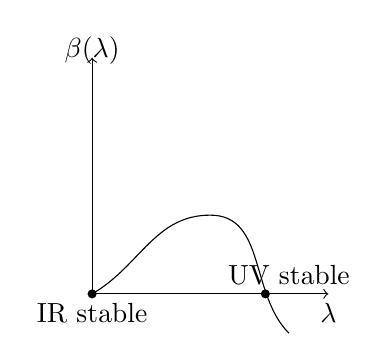
\begin{tikzpicture}[scale=1, transform shape, baseline]
   \draw [<->] (0,3) -- (0,0) -- (3,0);  
   \draw (0,0) to[out=30, in=180] (1.5,1) to[out=0, in=135] (2.5,-0.5);
   \node [right, anchor=base] at (0,3) {$\beta(\lambda)$};
   \node [below] at (3,0) {$\lambda$};

   \draw[fill] (0,0) circle [radius=0.05];
   \node [below] at (0,0) {IR stable};
   \draw[fill] (2.2,0) circle [radius=0.05];
   \node [above] at (2.5,0) {UV stable};
\end{tikzpicture}%
\begin{tikzpicture}[scale=1, transform shape, baseline]
   \draw [<->] (0,3) -- (0,0) -- (3,0);  
   \draw (0,0) to[out=-30, in=180] (1.5,-1) to[out=0, in=225] (2.5,0.5);
   \node [right, anchor=base] at (0,3) {$\beta(\lambda)$};
   \node [below] at (3,0) {$\lambda$};

   \draw[fill] (0,0) circle [radius=0.05];
   \node [above] at (0,0) {IR stable};
   \draw[fill] (2.2,0) circle [radius=0.05];
   \node [above] at (3.2,0) {UV stable};
\end{tikzpicture}
\end{center}
Non-perturbative zeros $\beta(\lambda_{NP}) = 0$ and perturbative $\beta(0)=0$ are fixed points for of RG flow. The second picture has \textit{asymptotic freedom} for $t \longmapsto \infty$, $\lambda(t) \longmapsto 0$ is a (UV-stable) fixed point; we believe QCD to have this property.
